\part{Programmation orientée-objets \\Design Patterns}
\section{Introduction}

Un Design Pattern est une solution à un problème récurrent dans la conception d’applications orientées objet. Un patron de conception décrit alors la solution éprouvée pour résoudre ce problème d’architecture de logiciel. Comme problème récurrent on trouve par exemple la conception d’une application où il sera facile d’ajouter des fonctionnalités à une classe sans la modifier (voir la solution du Design Pattern Visiteur). A noter qu’en se plaçant au niveau de la conception les Design Patterns sont indépendants des langages de programmation utilisés. 

Les Design Patterns sont représentés par :

\begin{itemize}
    \item Nom : qui permet de l’identifier clairement
    \item Problématique : description du problème auquel il répond
    \item Solution : description de la solution souvent accompagnée d’un schéma UML
    \item Conséquences : les avantages et les inconvénients de cette solution
\end{itemize}

L’utilisation des Design Patterns offre de nombreux avantages. Tout d’abord cela permet de répondre à un problème de conception grâce à une solution éprouvée et validée par des experts. Ainsi on gagne en rapidité et en qualité de conception ce qui diminue également les coûts. De plus, les Design Patterns sont réutilisables et permettent de mettre en avant les bonnes pratiques de conception.
Les Design Patterns étant largement documentés et connus d’un grand nombre de développeurs ils permettent également de faciliter la communication. Si un développeur annonce que sur ce point du projet il va utiliser le Design Pattern Observateur il est compris des informaticiens sans pour autant rentrer dans les détails de la conception.

Il existe trois sortes de design patterns: 
\begin{itemize}
    \item Création : permettent d’instancier et de configurer des classes et des objets
    \item Structure : permettent d’organiser les classes d’une application
    \item Comportement : permettent d'organiser les objets pour qu’ils collaborent entre eux de manière optimisée
\end{itemize}





\section{Factory Pattern}
\subsection{Problématique}
\begin{itemize}
    \item Catégorie : Creational Pattern
    \item Problème: créer un nouvel objet sans exposer la logique de création au client, et pouvoir créer des objets d'un type donné (interface, classe abstraite) sans fixer leur classe concrète
    \item Solution : Une méthode fabrique l’objet voulu (passé en argument) dans une autre classe
\end{itemize}
\subsection{Implémentation}
\begin{enumerate}
    \item Créer une interface qui regroupe toute les classes qu’on veut instancier
    \item Créer toutes les classes concrètes qu’on veut instancier
    \item Créer la classe Factory possédant la méthode (static) qui va prendre en argument l’ordre du client et qui va renvoyer l’objet voulu
    \item Créer le client

\end{enumerate}
\begin{figure}[!ht]
	\centering
	\begin{minipage}[t]{8.0cm}
		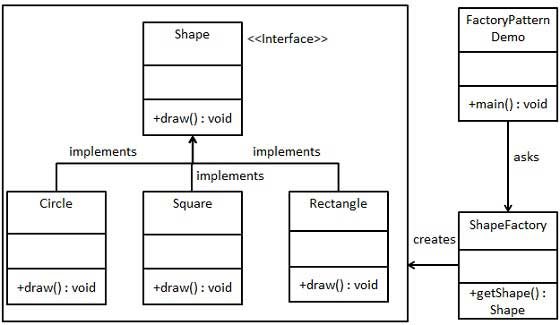
\includegraphics[scale=0.5]{Images/fact.jpg}
		\label{s1}
   		\caption{Structure du Factory Pattern}
	\end{minipage}
	
\end{figure}

\subsection{Discussions}

Ce pattern permet d'avoir plusieurs constructeurs (prenant d'autres arguments pour créer le même objet par exemple) regroupés dans une seule et même méthode factory.
Il permet d'instancier des objets dont le type est dérivé d'un type abstrait. La classe exacte de l'objet n'est donc pas connue par l'appelant.
Il est très souvent utilisé, comme par exemple la méthode java.awt.Color.make\_RGB\_color(r,g,b).



%------------------------------------


\section{Abstract Factory}
\subsection{Problématique}
\begin{itemize}
    \item Catégorie : Creational Pattern
    \item Problème : Créer des familles d'objets dépendants grâce à une même classe sans déterminer concrètement leur classe 
    \item Solution : Une "super Factory" qui crée d'autres Factories. Une interface est responsable de créer une usine à fabriquer des objets ayant des liens entre eux sans spécifier explicitement leurs classes. Chaque Factory peut retourner un nouvel objet (comme pour le Factory Pattern).
\end{itemize}
\subsection{Implémentation}
\begin{enumerate}
    \item Créer une abstract class (ou interface) AbstractFactory regroupant toutes les Factories d'objets qu'on veut créer
    \item Créer nos Factories implémentant AbstractFactory comme expliqué dans le Factory Pattern
    \item Créer une classe « FactoryProducer » qui selon l’argument appelle une autre factory qui elle va créer l’objet. Renvoie ensuite l’objet créé
    \item Créer le client dans lequel on utilise le FactoryProducer pour créer un AbstractFactory spécifique afin que le Factory concret crée l’objet qu’on veut
\end{enumerate}

\newpage
Exemple d'appel client: 
\begin{lstlisting}
    //get shape factory
  AbstractFactory shapeFactory = FactoryProducer.getFactory("SHAPE");

   //get an object of Shape Circle
  Shape shape = shapeFactory.getShape("CIRCLE");

   //call draw method of Shape Circle
  shape.draw();
\end{lstlisting}


\begin{figure}[!ht]
	\centering
	\begin{minipage}[t]{8.0cm}
		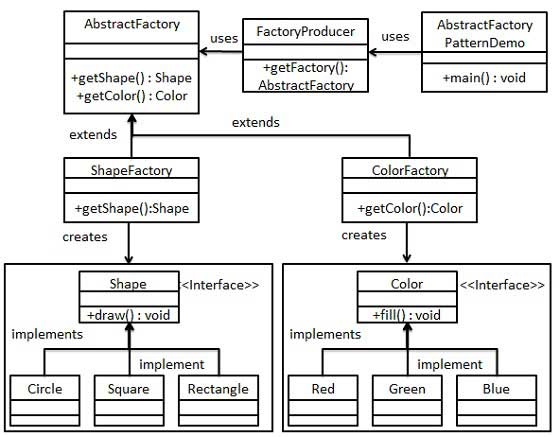
\includegraphics[scale=0.5]{Images/afact.jpg}
		\label{s1}
   		\caption{Structure de Abstract Factory Pattern}
	\end{minipage}
	
\end{figure}


\subsubsection{Discussions}
Avantage: Réduit	fortement	la	dépendance	sur	les	différentes	familles : seul	le module qui crée 
l'objet	Factory dépend des familles. \\
Inconvénient:L'objet Factory doit être transmis à tous les modules qui créent des objets de la famille. \\

Pour différencier Factory Method et Abstract Factory, on peut le voir comme ceci: le premier cache la construction d'un simple objet dans une méthode, alors que le deuxième cache la construction de toute une famille d'objets corrélés.  


%------------------------------------
\newpage
\section{Singleton}
\subsection{Problématique}
\begin{itemize}
    \item Catégorie : Creational Pattern
    \item Problème : On veut créer une classe avec une seule instance, globalement accessible.
    \item Solution : Créer et donner accès à une seule instance. Empêcher la création d'autres instances (constructeur privé).
\end{itemize}
\subsection{Implémentation}
\begin{enumerate}
    \item Créer la classe Singleton, avec le \textit{constructeur privé}, un attribut singleton = new Singleton() et une méthode getSingleton()
    \item Créer le client qui appelle getSingleton()

\end{enumerate}

\begin{figure}[!ht]
	\centering
	\begin{minipage}[t]{8.0cm}
		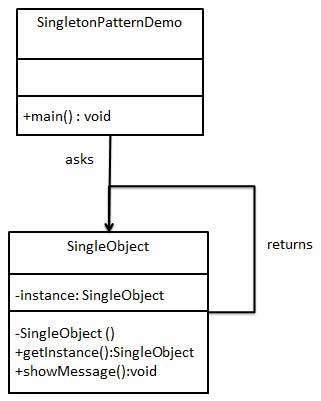
\includegraphics[scale=0.45]{Images/sing.jpg}
		\label{s1}
   		\caption{Structure du Singleton}
	\end{minipage}
	
\end{figure}


\subsection{Discussions}
Pratique pour créer un objet unique, et séparer ce code du reste du code par souci de clarté.





%------------------------------------






\section{FlyWeight }
\subsection{Problématique}
\begin{itemize}
    \item Catégorie : Structural Pattern
    \item Problème : Supporter un très grand nombre d'objets identiques (immutables). 
    \item Solution : Partager un seul objet pour toutes les instances identiques. Utiliser une méthode fabrique pour générer les instances. Distinguer l'état intrinsèque (immutable, invariable, stocké dans l'objet) et l'état extrinsèque (mutable, variable, passé en paramètre aux méthodes). 
\end{itemize}
\subsection{Implémentation}
\begin{enumerate}
    \item Créer une interface et une classe concrète l'implémentant 
    \item Créer une classe contenant une méthode Factory possédant un HashMap comme attribut: si l’objet avec la propriété passée en argument (= état immutable) n’existe pas encore, créer un nouvel objet et le renvoyer. Sinon, renvoyer un objet déjà créé en changeant uniquement son état extrinsèque.

\end{enumerate}

\begin{figure}[!ht]
	\centering
	\begin{minipage}[t]{8.0cm}
		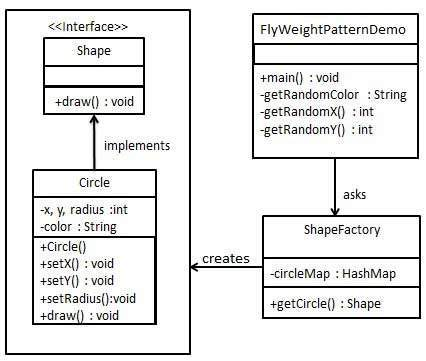
\includegraphics[scale=0.5]{Images/fly.jpg}
		\label{s1}
   		\caption{Exemple d'arborescence de FlyWeight Pattern}
	\end{minipage}
	
\end{figure}


\subsection{Discussions}
Il faut obligatoirement que l'objet ait un état intrinsèque, faute de quoi le pattern ne fonctionnera pas.
Exemple d'utilisation réelle: les String en Java.




%------------------------------------






\section{Composite}
\subsection{Problématique}
\begin{itemize}
    \item Catégorie : Structural Pattern
    \item Problème : Traiter un groupe d’objets de manière similaire à un unique objet
    \item Solution : Créer une classe contenant un groupe de ses propres objets. Cette classe fournit des manières de modifier ses groupes de mêmes objets. 
\end{itemize}
\subsection{Implémentation}
\begin{enumerate}
    \item Créer une classe Component dans laquelle il y a une liste d’instances de cette même classe. Cela permet également de représenter une forme de hiérarchie (ex : patron responsable de ("possédant") plusieurs employés, qui peuvent eux-même être responsable de ("posséder") plusieurs employés)
    \item ???
    \item Profit
\end{enumerate}

\begin{figure}[H]
	\centering
	\begin{minipage}[t]{8.0cm}
		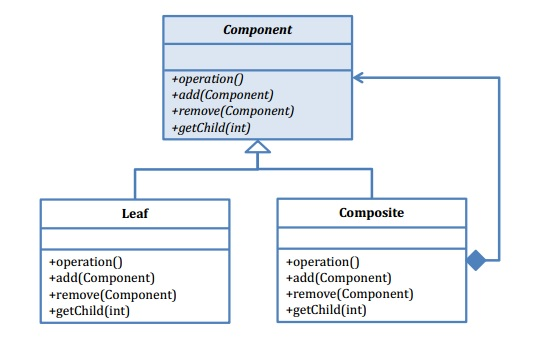
\includegraphics[scale=0.57]{Images/comp.jpg}
		\label{s1}
   		\caption{Structure de Composite Pattern}
	\end{minipage}
	
\end{figure}


\subsection{Discussions}
Permet de Simplifier les clients, car les composants primitifs et les conteneurs sont traités de la même manière.
On peut facilement ajouter des nouveaux types de composants.
Permet de maximiser les opérations offertes sur Component.





%------------------------------------





\section{Strategy}
\subsection{Problématique}
\begin{itemize}
    \item Catégorie : Behavioral Pattern
    \item Problème : Définir une famille de procédures encapsulées et interchangeables pour une fonctionnalité donnée, autrement dit donner la possibilité au code de choisir lui même l'algorithme d'exécution et/ou le comportement d'une classe.
    \item Solution : Une interface avec une méthode ayant un argument correspondant à la procédure choisie
\end{itemize}
\subsection{Implémentation}
\begin{enumerate}
    \item Créer une interface Strategy avec la méthode doOperation()
    \item Créer les classes concrètes implémentant Strategy avec des stratégies différentes (exemple: OperationAdd , OperationSubstract, OperationMultiply)
    \item Créer une classe Context qui prend une stratégie en argument dans son constructeur et possède une méthode executeStrategy()
    \item Créer le client qui n’a qu’à créer une instance de Context avec la stratégie qu’il veut en argument, puis exécuter la stratégie 

\end{enumerate}
Exemple de client : 
\begin{lstlisting}
    Context context = new Context(new OperationAdd());		
    System.out.println("10 + 5 = " + context.executeStrategy(10, 5));
\end{lstlisting}


\begin{figure}[H]
	\centering
	\begin{minipage}[t]{8.0cm}
		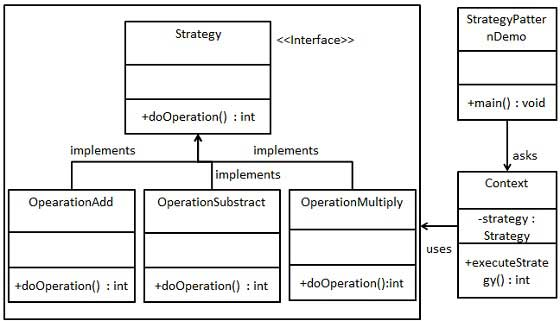
\includegraphics[scale=0.4]{Images/strat.jpg}
		\label{s1}
   		\caption{Exemple d'arborescence du Strategy Pattern}
	\end{minipage}
	
\end{figure}


\subsection{Discussions}
L'utilité de ce pattern est de séparer des algorithmes différents dans différentes classes qui pourront être choisis et exécutés au moment de l'exécution, en plus de garder une clarté dans le code.
Un exemple très connu est la méthode compareTo() dans Object en Java.





%------------------------------------




\section{Command}
\subsection{Problématique}
\begin{itemize}
    \item Catégorie : Behavioral Pattern
    \item Problème : Définir une famille de requêtes encapsulées et interchangeables pour des comportements quelconques 
    \item Solution : Une interface avec une méthode correspondant à la requête
\end{itemize}
\subsection{Implémentation}
\begin{enumerate}
    \item Créer une interface Commande (Order) qui ne possède que quelques méthodes (execute() au minimum; undo() et redo() sont aussi généralement utilisées)
    \item Créer une classe concrète Receiver qui correspond à l’objet qui subira la commande/l’action (exemples: télévision, document)
    \item Créer des classes concrètes implémentant Commande, chacune représentant une commande particulière dépendant du Receiver (exemples:: télévision : on/off/volumeUp/volumeDown ; document : save/open )
    \item Créer une classe Invoker, qui possède une liste de commandes et peut soit en rajouter soit les exécuter (la liste n'est pas obligatoire mais permet de retenir les commandes et donc d'implémenter les undo/redo)
    \item Créer la classe Client, qui instancie des nouvelles commandes, peut les rajouter à la liste du Invoker et les exécuter quand il veut.

\end{enumerate}
\newpage
Exemple d'appel de client: 
\begin{lstlisting}
    Television tv = new Television();

    TvOn tvOnOrder = new TvOn(tv);
    TvVolumeUp tvUpOrder = new TvVolumeUp(tv);
    
    Invoker button = new Invoker();
    button.takeOrder(tvOnOrder);
    button.takeOrder(tvUpOrder);
    
    button.executeOrders();
\end{lstlisting}


\begin{figure}[H]
	\centering
	\begin{minipage}[t]{8.0cm}
		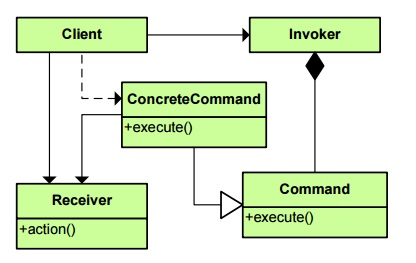
\includegraphics[scale=0.7]{Images/comm.jpg}
		\label{s1}
   		\caption{Structure de Command Pattern}
	\end{minipage}
	
\end{figure}

\subsection{Discussions}

La commande n'a pas de résultat mais produit un effet. Les données du contexte sont fournies à la construction de la commande. Permet d'éviter des conditionnelles. Les commandes peuvent être postposées, mises en files, transférées, rejouées, … Supporte undo avec une méthode supplémentaire



%------------------------------------






\section{Observer}
\subsection{Problématique}
\begin{itemize}
    \item Catégorie : Behavioral Pattern
    \item Problème : Définir un lien entre objets tel que quand un objet est modifié, les objets dépendants soient notifiés. 
    \item Solution : C'est le sujet qui invoque observer.update() dans une méthode notifyChanges(), au lieu de l'observer qui vient demander si un changement a été apporté
\end{itemize}
\subsection{Implémentation}
\begin{enumerate}
    \item Créer une interface Observer contenant la méthode update() et les classes concrètes l'implémentant
    \item Créer l’interface Subject contenant 3 méthodes : attach() / detach() ( = s'abonner ou se désabonner aux notifications) et notify() (appelle les méthodes update() de tous les observers abonnés)
    

\end{enumerate}

\begin{figure}[!ht]
	\centering
	\begin{minipage}[t]{8.0cm}
		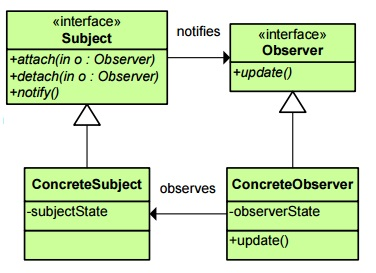
\includegraphics[scale=0.7]{Images/obs.jpg}
		\label{s1}
   		\caption{Structure de Observer Pattern}
	\end{minipage}
	
\end{figure}


\subsection{Discussions}
Ce pattern est beaucoup utilisé pour tout ce qui est interaction avec l'interface graphique (boutons, editTexts, etc.). Il permet de gagner du temps et de la mémoire, car sans cette méthode, les observateurs devraient vérifier toutes les x secondes si un changement a été apporté. \\
Voici un exemple concret pour mieux comprendre ce pattern. Considérer le subject comme un reporter freelance ayant pour rôle de dénicher des scoops et les Observers comme des grandes chaînes de télévision (Rtbf, RTL, ...). Le principe du pattern est que lorsqu'il a un scoop, le reporter prévient toutes les chaînes qui le paient pour avoir des scoops. Or sans ce pattern, les chaînes ne cesseraient d'appeler le reporter pour demander s'il y a du nouveau, ce qui est une grande perte de temps pour les deux partis.






%------------------------------------






\section{Interpreter}
\subsection{Problématique}
\begin{itemize}
    \item Catégorie : Behavioral Pattern
    \item Problème : Définir un calcul sur une structure arborescente (représentant les phrases d'un langage). Convertir une représentation de données en une autre représentation des mêmes données. Parcourir un arbre d’interprétation en effectuant un certain calcul (Plusieurs calculs différents (évaluer, imprimer, …) + le calcul dépend du type de noeud )
    \item Solution : Une méthode interpret sur toutes les classes de l'arborescence + TerminalExpression (=leaf) et CompoundExpression(= noeud)
\end{itemize}
\subsection{Implémentation}
\begin{enumerate}
    \item Créer une classe abstraite (ou interface) Expression contenant une méthode interpret()
    \item Créer des classes terminales TerminalExpression implémentant Expression, attribuant une valeur finale (leaf) à l’expression passée en argument. Ces classes permettent de traiter les plus petits morceaux de l'information reçue (si on a par exemple (a \&\& b) comme entrée, les deux 'leaves' ou plus petites parties sont a et b, et TerminalExpression.interpret(a) devrait renvoyer true si a==true et false sinon )
    \item Créer d’autres classes implémentant Expression, toutes composites (voir le Design Pattern Composite) et appelant les méthodes interpret() de chaque expression (en continuant dans le même exemple, on pourrait par exemple avoir OrExpression ou AndExpression)
    \item Créer les classe concrètes Client et Contexte (dans l'exemple ci-dessus le contexte serait des Boolean).

\end{enumerate}

\begin{figure}[!ht]
	\centering
	\begin{minipage}[t]{8.0cm}
		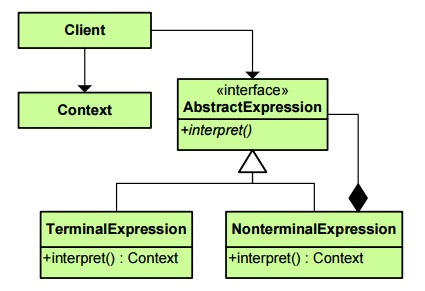
\includegraphics[scale=0.65]{Images/int.jpg}
		\label{s1}
   		\caption{Structure de Interpreter Pattern}
	\end{minipage}
	
\end{figure}


\subsection{Discussions}
Ce pattern est basé sur le patron Composite et est le plus souvent utilisé pour interpréter un langage, mais il reste applicable à tout autre type de structure composée. Il permet l'extension facile d'un langage ou l'ajout de fonctions d'interprétation difficiles (une méthode par classe du langage). Egalement utilisé lorsqu’un logiciel doit analyser/parser une chaîne algébrique (= expression) ou lorsqu’un logiciel doit produire différents types de données comme résultat.




%------------------------------------






\section{Visitor}
\subsection{Problématique}
\begin{itemize}
    \item Catégorie : Behavioral Pattern
    \item Problème : Définir plusieurs calculs basée sur une seule structure, sans changer les classes de la structure. Séparer un algorithme d’une structure de données
    \item Solution : ElementA.accept(v) appelle visitElementA(this)
\end{itemize}
\subsection{Implémentation}
\begin{enumerate}
    \item Créer une interface Visitable (ou Element) contenant la méthode accept(Visitor v)
    \item Créer les classes concrètes implémentant Visitable, les méthodes accept() faisant appel à v.visit(this)
    \item Créer une interface Visitor contenant toutes les méthodes visit(Visitable v)
    \item Créer une classe ConcreteVisitor implémentant Visitor et toutes ses méthodes

\end{enumerate}



\begin{figure}[!ht]
	\centering
	\begin{minipage}[t]{8.0cm}
		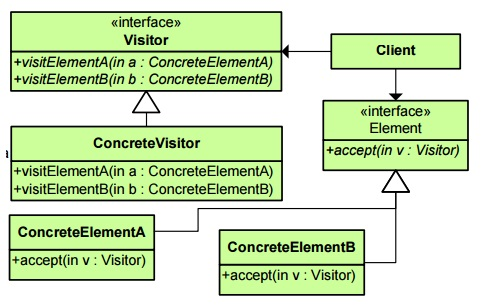
\includegraphics[scale=0.65]{Images/vis.jpg}
		\label{s1}
   		\caption{Structure de Visitor Pattern}
	\end{minipage}
	
\end{figure}


\subsection{Discussions}
Ce pattern est très pratique lorsqu’on veut ajouter une fonctionnalité sans trop modifier le code de base par souci de clarté (exemple: le débuggage). Il peut s'appliquer à toute structure, pas uniquement les Composite. On peut mettre le parcours de la structure dans le visiteur. On a un parcours plus précis en fonction du calcul (+++), mais répété pour chaque visiteur (---).

